% !TeX program = lualatex
% fourier.tex 第2節の補助教材。ビルド: lualatex fourier2.tex（2回）
\documentclass[a4paper,11pt]{article}
\usepackage{luatexja}
\usepackage[haranoaji]{luatexja-preset}
\usepackage{amsmath,amssymb,booktabs,array}
\usepackage[margin=22mm,top=20mm,bottom=21mm]{geometry}
\usepackage{xcolor,tikz,pgfplots}
\usepackage{enumitem,fancyhdr}
\usepackage[unicode,hidelinks]{hyperref}
\pgfplotsset{compat=1.18}
\definecolor{main}{HTML}{165678}
\definecolor{accent}{HTML}{B04A27}
\definecolor{pale}{HTML}{EEF5F8}
\setlength{\parindent}{1em}
\setlength{\parskip}{5pt}
\renewcommand{\baselinestretch}{1.16}
\setlist{nosep,leftmargin=2em}
\pagestyle{fancy}\fancyhf{}
\fancyhead[L]{\small フーリエ級数からフーリエ変換へ}
\fancyhead[R]{\small 高専生向け補助教材}
\fancyfoot[C]{\thepage}
\setlength{\headheight}{16pt}
\newcommand{\heading}[2]{\vspace*{2mm}{\Large\bfseries\color{main}#1\quad #2}\par\vspace{3mm}}
\newcommand{\sub}[1]{\par\vspace{2mm}{\bfseries\color{main}#1}\par}
\newcommand{\point}[1]{\par\smallskip\noindent\colorbox{pale}{\parbox{\dimexpr\linewidth-2\fboxsep\relax}{\strut #1\strut}}\par\smallskip}
\newcommand{\ii}{\mathrm{i}}
\begin{document}
\heading{1}{繰り返す波から，1回だけの波へ}
\noindent 本資料は \texttt{fourier.tex} 第2節「フーリエ級数からフーリエ変換へ」を解説する補助教材です。三角関数，複素数，積分の基礎を使い，元資料の式(6)〜(12)を順に読み解きます。

\sub{フーリエ級数で学んだこと}
複雑な波も，振動の速さが異なる単純な波を足し合わせて表せます。周期 $T$ の波を複素数で表すと，
\[
 f(t)=\sum_{n=-\infty}^{\infty}c_n e^{\ii n\omega_0t},
 \qquad \omega_0=\frac{2\pi}{T},\qquad \ii^2=-1
\]
です。$\sum$ は「各項を足す」という記号，$c_n$ は各成分の大きさと位相を決める複素数です。Eulerの公式
\[
 e^{\ii\theta}=\cos\theta+\ii\sin\theta
\]
によって，指数関数で書いた波も三角関数と結びつきます。

\sub{1回だけの衝撃も調べたい}
機械を一度たたいたときの振動や，短時間だけ出る電圧は，通常は同じ形をいつまでも繰り返しません。このような信号を考えるため，まず $[-T/2,T/2]$ の波形を取り出して，周期 $T$ で繰り返すと考えます。
\begin{center}
\begin{tikzpicture}[x=0.78cm,y=0.8cm]
\draw[->] (-8,0)--(8,0) node[right] {$t$};
\foreach \c in {-6,0,6}{\draw[main,thick] (\c-0.65,0)--(\c-0.65,1)--(\c+0.65,1)--(\c+0.65,0);}
\draw[<->] (0,1.5)--(6,1.5) node[midway,above] {$T$};
\node[left] at (-8,0.5) {\small 繰り返し};
\begin{scope}[yshift=-2.8cm]
\draw[->] (-8,0)--(8,0) node[right] {$t$};
\draw[accent,thick] (-0.65,0)--(-0.65,1)--(0.65,1)--(0.65,0);
\node[left] at (-8,0.5) {\small 1回だけ};
\node[below] at (0,0) {$0$};
\end{scope}
\end{tikzpicture}
\end{center}
$T$ を大きくすると，隣の繰り返しは遠くへ離れます。$T\to\infty$（$T$ を限りなく大きくする）と，中央の波形を1回だけ取り出した状況に近づきます。\textbf{波形を横に引き伸ばすのではなく，考える区間を広げる}のがポイントです。
\point{フーリエ変換への道筋は，\textbf{「時間の区間を無限に広げ，周波数ごとの足し算を積分に変える」}ことです。ここでは，短いパルスのように積分を扱える信号で考えます。}

\newpage
\heading{2}{区間が長くなると，周波数の間隔は狭くなる}
\sub{なぜ $\omega_n=n\,2\pi/T$ なのか：元資料の式(8)，(9)}
区間 $T$ にちょうど $n$ 回の振動が入る波は，周波数が $\nu_n=n/T$ Hzです。本資料では，信号 $f(t)$ と区別するため，周波数に $\nu$ を使います。1周は $2\pi$ radなので，角周波数は
\[
 \omega_n=2\pi\nu_n=n\frac{2\pi}{T}.
\]
隣り合う角周波数の差は
\[
 \boxed{\Delta\omega=\omega_{n+1}-\omega_n=\frac{2\pi}{T}=\omega_0}.
\]
\begin{center}
\begin{tabular}{ccc}
\toprule
区間の長さ $T$ [s] & 周波数の間隔 $\Delta\nu=1/T$ [Hz] & $\Delta\omega$ [rad/s]\\\midrule
1 & 1 & $2\pi$\\
2 & 0.5 & $\pi$\\
4 & 0.25 & $\pi/2$\\
10 & 0.1 & $\pi/5$\\\bottomrule
\end{tabular}
\end{center}
\sub{周波数の目盛りが細かくなる様子}
\begin{center}
\begin{tikzpicture}[x=2.4cm,y=1cm]
\foreach \y/\lab in {2/{T=1\ \mathrm{s}},1/{T=2\ \mathrm{s}},0/{T=4\ \mathrm{s}}}{
\draw[->] (-2.15,\y)--(2.25,\y);
\node[left] at (-2.2,\y) {$\lab$};}
\foreach \x in {-2,-1,...,2}{\fill[main] (\x,2) circle (2pt);}
\foreach \x in {-2,-1.5,...,2}{\fill[main] (\x,1) circle (2pt);}
\foreach \x in {-2,-1.75,...,2}{\fill[accent] (\x,0) circle (2pt);}
\foreach \x in {-2,-1,0,1,2}{\node[below] at (\x,-0.15) {$\x$};}
\node[below] at (0,-0.65) {周波数 $\nu$ [Hz]};
\end{tikzpicture}
\end{center}
点は「フーリエ級数で使う周波数の位置」を示し，成分の大きさを示しているわけではありません。$T$ が大きいほど，点の間隔が狭くなります。
\[
 T\to\infty\quad\Longrightarrow\quad\Delta\omega\to0.
\]
この極限で，飛び飛びだった周波数を連続した変数 $\omega$ として扱います。$n$ は周波数の\textbf{番号}ですが，$\omega$ は周波数の\textbf{値}です。

\sub{負の周波数は何を表すのか}
$\cos\theta=(e^{\ii\theta}+e^{-\ii\theta})/2$ のように，実数の波を複素数で表すと，正負の周波数が対になります。「負の回数で振動する」という意味ではなく，複素数の回転方向を区別するための表現です。

\newpage
\heading{3}{係数を置き換えると，フーリエ変換が現れる}
\sub{まず $c_n$ の式を確認する}
元資料の式(5)で，積分区間を $[-T/2,T/2]$ に選ぶと，
\[
 c_n=\frac1T\int_{-T/2}^{T/2}f(t)e^{-\ii n\omega_0t}\,dt.
\]
波形に調べたい周波数の波を掛け，1周期分を積分することで，その成分の係数を求めています。

\sub{$1/T$ を外した量を $X_n$ とする：式(6)，(7)}
\point{元資料は，新しい量を次のように定義しています。
\[
 X_n=\int_{-T/2}^{T/2}f(t)e^{-\ii n\omega_0t}\,dt
 \qquad\Longrightarrow\qquad X_n=Tc_n.
\]}
したがって，$c_n=X_n/T$ を級数に代入すれば，
\[
 f(t)=\frac1T\sum_{n=-\infty}^{\infty}X_n e^{\ii n\omega_0t}
\]
となります。この段階では，係数の書き方を変えただけです。

\sub{なぜ，わざわざ $1/T$ を外すのか}
幅が決まった1回だけのパルスを考えると，区間を長くしても，パルス自体は変わりません。一方，$c_n$ には $1/T$ があるので，固定した周波数付近の係数は小さくなります。周波数の間隔が狭くなって成分の数が増えるため，\textbf{係数をそのまま比べるより，$T$ 倍した $X_n$ を使うと極限を考えやすい}のです。

\sub{積分区間を実数全体へ広げる：式(10)}
$n\omega_0$ を連続した角周波数 $\omega$ に置き換え，区間を広げると，
\[
 \boxed{X(\omega)=\int_{-\infty}^{\infty}f(t)e^{-\ii\omega t}\,dt}
\]
を得ます。これが\textbf{フーリエ変換}です。各 $\omega$ を指定すると，1つの複素数 $X(\omega)$ が計算できます。

番号 $n$ を固定したまま $T\to\infty$ にすると $n\omega_0\to0$ になります。ここで考えているのは，\textbf{調べたい $\omega$ に近い格子点を，$T$ ごとに選んでいく}ことです。
\point{積分は時間 $t$ について行います。計算が終わると $t$ は残らず，指定した角周波数 $\omega$ に応じた答え $X(\omega)$ が残ります。信号が電圧 [V] なら，$X(\omega)$ の単位は [V$\cdot$s] です。}

\newpage
\heading{4}{「足し算」が「積分」になる仕組み}
\sub{$1/T$ を周波数の間隔で書く：元資料の式(11)}
$\Delta\omega=2\pi/T$ を変形すると，
\[
 \frac1T=\frac{\Delta\omega}{2\pi}.
\]
これを前ページの級数に入れ，$\omega_n=n\omega_0$ と書けば，
\[
 f(t)=\frac1{2\pi}\sum_{n=-\infty}^{\infty}
 \underbrace{X_n e^{\ii\omega_n t}}_{\text{各周波数での値}}
 \underbrace{\Delta\omega}_{\text{周波数の幅}}
\]
です。ここで\textbf{「値 $\times$ 小さな幅」の足し算}が現れました。

\sub{定積分を，長方形の面積で思い出す}
普通の関数 $g(\omega)$ の積分では，次の近似を使います。
\[
 \int_a^b g(\omega)\,d\omega
 \ \approx\ \sum_n g(\omega_n)\Delta\omega.
\]
\begin{center}
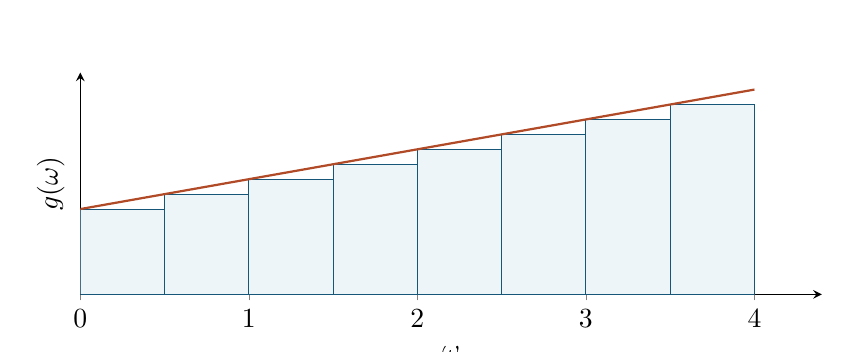
\begin{tikzpicture}
\begin{axis}[width=11cm,height=4.4cm,xmin=0,xmax=4.4,ymin=0,ymax=2.6,
 axis lines=left,xlabel={$\omega$},ylabel={$g(\omega)$},xtick={0,1,2,3,4},ytick=\empty]
\addplot[ybar interval,fill=pale,draw=main] coordinates {(0,1) (0.5,1.175) (1,1.35) (1.5,1.525) (2,1.7) (2.5,1.875) (3,2.05) (3.5,2.225) (4,2.4)};
\addplot[accent,thick,domain=0:4]{1+0.35*x};
\end{axis}
\end{tikzpicture}
\end{center}
幅 $\Delta\omega$ を小さくすると，長方形の面積の和が積分に近づきます。複素数を値に持つ関数でも，実部と虚部をそれぞれ積分すれば，同じ考え方が使えます。

\sub{周波数について積分すると元の波になる：式(12)}
$T\to\infty$ で，$X_n$ を $X(\omega)$，足し算を積分に移すと，
\point{\textbf{逆フーリエ変換}
\[
 \boxed{f(t)=\frac1{2\pi}\int_{-\infty}^{\infty}
 X(\omega)e^{\ii\omega t}\,d\omega}
\]}
順変換は\textbf{時間について積分して成分を調べる}計算，逆変換は\textbf{周波数について積分して波を組み立てる}計算です。$1/(2\pi)$ は突然付けた係数ではなく，$1/T=\Delta\omega/(2\pi)$ から出てきます。
\noindent{\small ※ここでは極限への移り方を直感的に説明しています。復元が成り立つ条件の詳しい証明は省略します。区分的に滑らかな信号の跳びの点では，逆変換は左右の値の平均を与えます。}

\newpage
\heading{5}{計算例：短時間だけ出る電圧を変換する}
\sub{高さ $A$，幅 $\tau$ のパルス}
$A>0$，$\tau>0$ とし，時間原点を中心とした信号を考えます。$\tau$ は\textbf{パルスの幅}であり，これまでの区間の長さ $T$ とは別です。
\[
 f(t)=\begin{cases} A,&|t|<\tau/2,\\0,&|t|>\tau/2.\end{cases}
\]
端点2か所の値は積分結果に影響しません。電気回路に加える短い電圧を単純化した例です。
\sub{波がある区間だけ積分する}
$\omega\ne0$ なら，
\begin{align*}
 X(\omega)
 &=A\int_{-\tau/2}^{\tau/2}e^{-\ii\omega t}\,dt\\
 &=A\left[\frac{e^{-\ii\omega t}}{-\ii\omega}\right]_{-\tau/2}^{\tau/2}
 =A\frac{e^{-\ii\omega\tau/2}-e^{\ii\omega\tau/2}}{-\ii\omega}\\
 &=\frac{2A\sin(\omega\tau/2)}{\omega}
 =\boxed{A\tau\frac{\sin(\omega\tau/2)}{\omega\tau/2}}.
\end{align*}
最後の変形では $e^{-\ii u}-e^{\ii u}=-2\ii\sin u$ を使いました。$\omega=0$ は元の積分から計算すれば，
\[
 X(0)=\int_{-\tau/2}^{\tau/2}A\,dt=\boxed{A\tau}
\]
です。これはパルスの面積です。$\sin u/u\to1$ という極限でも同じ値になります。
\begin{center}
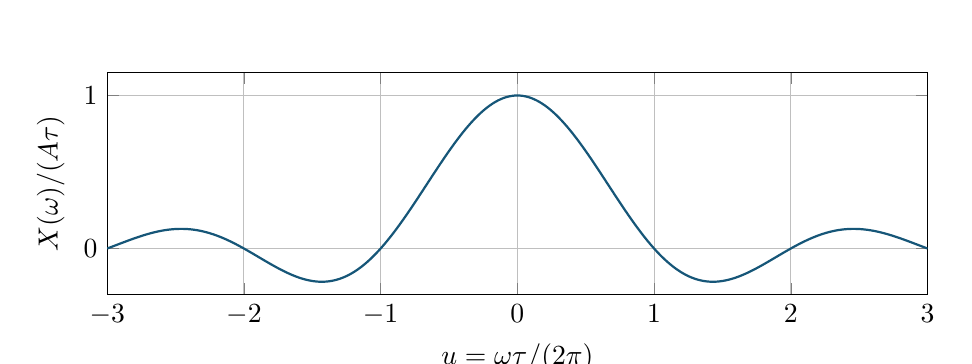
\begin{tikzpicture}
\begin{axis}[width=12cm,height=4.4cm,xmin=-3,xmax=3,ymin=-0.3,ymax=1.15,
 xlabel={$u=\omega\tau/(2\pi)$},ylabel={$X(\omega)/(A\tau)$},xtick={-3,-2,-1,0,1,2,3},ytick={0,1},grid=major]
\addplot[main,thick,domain=-3:3,samples=301]{abs(x)<0.00001 ? 1 : sin(deg(pi*x))/(pi*x)};
\end{axis}
\end{tikzpicture}
\end{center}
\point{1回だけの短いパルスにも，幅広い周波数の成分が含まれます。最初に0になる正の角周波数は $\omega=2\pi/\tau$。\textbf{パルスが短いほど，スペクトルの中央の山は横に広がります。}}
図は絶対値ではなく $X(\omega)$ 自体を描いています。この信号は左右対称なので変換は実数になり，負の部分は位相 $\pi$ に対応します。

\newpage
\heading{6}{Q10の答えと，理解の確認}
\sub{フーリエ成分 $X(\omega)$ は何を意味するか}
\point{\textbf{Q10の解答例：}フーリエ成分 $X(\omega)$ は，信号を周波数ごとの波に分けて見たときの，成分の大きさと位相の情報を表す複素数である。絶対値 $|X(\omega)|$ は成分の大きさを，偏角は余弦波を基準にした位相のずれを表す。これらの成分を逆フーリエ変換で重ね合わせると，元の信号が得られる。}
例えば音なら，「どの高さの音の成分が強いか」が絶対値から分かります。位相は波の山や谷が現れるタイミングに関係します。$X(\omega)=0$ のところでは位相は決められません。

\sub{絶対値をそのまま1本の波の振幅にしてよいか}
級数では，正負の対を合わせた実数の振動の振幅は $2|c_n|$ でした。ここで $c_n=X_n\Delta\omega/(2\pi)$ なので，
\[
 2|c_n|=\frac{|X_n|}{\pi}\Delta\omega.
\]
変換では周波数が連続するため，\textbf{小さな周波数の幅と組み合わせて，波への寄与を考えます。}$|X(\omega)|$ 自体が1本の波の振幅になるわけではありません。例えば電圧信号なら，振幅は V，$X$ は V$\cdot$s で，単位も異なります。

\sub{元資料の式のつながり}
\begin{center}
\begin{tabular}{cl}
\toprule
元資料の式 & 行っていること\\\midrule
(6)，(7) & $X_n=Tc_n$ と置き，級数の係数を書き換える。\\
(8)，(9) & 周波数が $\Delta\omega=2\pi/T$ 刻みで並ぶと確認する。\\
(10) & 時間区間を広げ，フーリエ変換 $X(\omega)$ を得る。\\
(11) & $1/T=\Delta\omega/(2\pi)$ で，積分に移れる形にする。\\
(12) & 周波数の和を積分に変え，逆フーリエ変換を得る。\\\bottomrule
\end{tabular}
\end{center}
\sub{確認問題}
\begin{enumerate}[label=(\arabic*)]
\item $T=5$ sのとき，$\Delta\nu$ [Hz] と $\Delta\omega$ [rad/s] を求めよ。
\item $T$ を2倍にすると，周波数の間隔はどうなるか。
\item 高さ2 V，幅0.1 sの中央対称なパルスについて，$X(0)$ と，最初に $X$ が0になる正の周波数 $\nu$ を求めよ。
\end{enumerate}
\sub{解答}
\noindent (1) $\Delta\nu=1/5=0.2$ Hz，$\Delta\omega=2\pi/5$ rad/s。\\
(2) $\Delta\omega=2\pi/T$ より半分になる。\\
(3) $X(0)=A\tau=0.2$ V$\cdot$s。$\omega=2\pi/\tau$ より $\nu=1/\tau=10$ Hz。
\end{document}
